\section{Introduction}\label{sec:intro}

The $n$-queens problem asks how to place $n$ queens on an $n\times n$ board so that no two share a row, column, or diagonal of either
slope. Once we have placed $q$ queens, exactly $n-q$ rows and $n-q$ columns remain empty. On a board of size $5\times5$ with four
queens, for example, the empty row and column determine a single candidate square. In Figure~\ref{fig:tablero-fibras}(a), both
diagonals through that square are also free, so the fifth queen can be placed there. We number rows and columns starting at zero and
give the row first.

\begin{figure}[htbp]
\centering
\begin{tikzpicture}[font=\small]
\begin{scope}[x=.51cm,y=-.51cm]
  \fill[black!4] (0,0) rectangle (5,5);
  \fill[teal!18] (0,2) rectangle (5,3);
  \fill[teal!18] (2,0) rectangle (3,5);
  \foreach \i in {0,...,5}{
    \draw[black!48,thin] (0,\i) -- (5,\i);
    \draw[black!48,thin] (\i,0) -- (\i,5);
  }
  \foreach \i in {0,...,4}{
    \node[left] at (0,\i+.5) {\scriptsize\i};
    \node[above] at (\i+.5,0) {\scriptsize\i};
  }
  \foreach \r/\c in {0/1,1/4,3/0,4/3}{
    \fill (\c+.5,\r+.5) circle[radius=2.7pt];
  }
  \draw[teal!65!black,line width=.9pt] (2.5,2.5) circle[radius=3.1pt];
  \node[anchor=north] at (2.5,5.25) {(a) A $5\times5$ board};
\end{scope}
\begin{scope}[shift={(5.15,0)},x=2.55cm,y=-2.55cm]
  \draw[black!60] (0,0) rectangle (1,1);
  \draw[teal!65!black,thick] (0,0) -- (1,1);
  \draw[teal!65!black,thick,dashed] (0,.5) -- (.5,1);
  \node[fill=white,inner sep=1pt,font=\scriptsize] at (.61,.59) {$r-c=0$};
  \node[fill=white,inner sep=1pt,font=\scriptsize] at (.25,.77) {$r-c=\tfrac12$};
  \node[left] at (0,0) {$0$}; \node[left] at (0,1) {$1$};
  \node[above] at (1,0) {$1$};
  \node[above] at (.50,0) {column $c$};
  \node[rotate=90] at (-.20,.50) {row $r$};
  \node[anchor=north] at (.5,1.05) {(b) Unit square};
\end{scope}
\end{tikzpicture}
\caption{From the board to the lines of the unit square. In (a), each black dot represents a queen.
Row~2 and column~2 are empty. The circle marks their intersection.
In (b), each value of $r-c$ identifies a diagonal. Its projection onto the row axis has
length one for the solid line and one half for the dashed line.}
\label{fig:tablero-fibras}
\end{figure}

Assign mass $1/n$ to each queen. The placement has total mass $\rho=q/n$, and $x=1-\rho$ is the fraction of empty rows, which equals
the fraction of empty columns. In the example, $x=1/5$. On passing to the unit square, we can ask how the mass is distributed if we
retain the capacity constraint for each family of lines. On a full board ($\rho=1$, $x=0$), the rows and columns use up their capacity.
What information about their distribution survives as we approach this endpoint through partial masses?

At mass one, Simkin~\cite{Simkin} related the entropy of a profile on the square to the number $Q(n)$ of solutions and obtained
$Q(n)=((1+o(1))\,n\,e^{-\alpha})^n$. Nobel, Agrawal, and Boyd~\cite{NAB} showed that $\alpha$ lies between $1.944000752$ and
$1.944001082$. Here we study how the entropy-maximizing profile varies as $\rho$ increases to one. To distinguish two rows whose
remaining capacities both tend to zero, we measure the share of the total vacancy attributable to each row.

\subsection{The continuous problem}


Consider the square $[0,1]^2$, with row and column coordinates $(r,c)$. The four families of lines are the rows, columns, diagonals, and
antidiagonals, with projections \[
 \ell_R(r,c)=r,\qquad \ell_C(r,c)=c,\qquad \ell_D(r,c)=r-c,\qquad \ell_A(r,c)=r+c,
\] taking values in $I_R=I_C=[0,1]$, $I_D=[-1,1]$, and $I_A=[0,2]$. For a density $\nu\ge0$ on the square, $m_f$ denotes its projection
onto the family $f$ and $u_f=1-m_f$ its \emph{vacancy}, or remaining capacity. For example, $m_R(r)$ is obtained by integrating
$\nu(r,c)$ with respect to $c$ along the row $r$. On a diagonal, the integral runs only over the segment inside the square
(Figure~\ref{fig:tablero-fibras}(b) and Section~\ref{sec:preliminares}). For $\rho\in(0,1]$, the admissible class $\cA_\rho$ consists
of the densities of mass $\rho$ such that $m_f\le1$ almost everywhere for all four families, and \begin{equation}\label{eq:funcional}
 s[\nu]=-3\rho-\int_{[0,1]^2}\nu\log\nu-\sum_{f\in\{R,C,D,A\}}\int_{I_f}u_f\log u_f,\qquad
 \sopt(\rho)=\sup_{\nu\in\cA_\rho}s[\nu].
\end{equation}

The first integral measures how the mass is distributed over the square. The other four terms describe how the remaining capacity is
distributed within each family. At mass one, the row and column vacancies vanish and $s$ coincides with the entropy in Simkin's problem
(Remark~\ref{obs:simkin}). By the \emph{optimal profile} we mean the density that maximizes $s$ at a given mass, together with its four
projections.

\subsection{Main results}

\begin{teorema}[Maximizer and Euler equation]\label{thm:euler} For each $\rho\in(0,1)$, $s$ attains its supremum over $\cA_\rho$ at a
unique density $\nu_\rho$, and there exists $\lambda=\lambda(\rho)>0$ such that \[
 \nu_\rho=\lambda\prod_f u_f\circ\ell_f\quad\text{almost everywhere},\qquad
 \frac{\lambda}{(1+\lambda)^4}\le\nu_\rho\le\lambda,\qquad m_f\le\frac{\lambda}{1+\lambda}.
\] The function $\sopt$ is strictly concave and differentiable on $(0,1)$, with $\sopt{}'(\rho)=-\log\lambda(\rho)$. The function
$\lambda$ is continuous and strictly increasing, with $\lambda\to0$ as $\rho\to0$ and $\lambda\to\infty$ as $\rho\to1$. For $\rho=1$,
the supremum is also attained at a unique density $\nu_1$. \end{teorema}

The Euler equation relates the density at a square to the remaining capacities of the four lines through it. The constant $\lambda$,
which we call the \emph{activity}, adjusts the total mass. As $\rho$ tends to one, $\lambda$ grows without bound and the row and column
vacancies each have integral $x$. To retain their spatial distribution we write, with $\rho=1-x\in(0,1)$,
\begin{equation}\label{eq:reescala}
 r_R=\frac{u_R}x,\qquad r_C=\frac{u_C}x,\qquad b=\lambda x^2,
\end{equation} so that $\nu=b\,r_R\,r_C\,u_D\,u_A$ and $\int_0^1r_R=\int_0^1r_C=1$.

\begin{teorema}[The profile near the full board]\label{thm:lleno} There exist explicit constants $0<\kappa\le1$, $1\le M<\infty$, and
$0<b_+<\infty$ such that, for every $x\in(0,1/2]$, \[
 \tfrac12\le b\le b_+,\qquad \frac1{1+b_+}\le r_R,r_C\le M,\qquad \kappa\le u_D,u_A\le1 .
\] As $x\downarrow0$, $(b,r_R,r_C,u_D,u_A)$ converges uniformly to a limit $(b_0,r_{R,0},r_{C,0},u_{D,0},u_{A,0})$ consisting of
positive continuous functions, with $\nu_1=b_0\,r_{R,0}\,r_{C,0}\,u_{D,0}\,u_{A,0}$, and the map $x\mapsto(\log r_R,\log r_C,\log
u_D,\log u_A,\log b)$, taking values in $\bigoplus_fC(I_f)\times\mathbb R$, extends analytically to a neighborhood of $x=0$.
\end{teorema}
